\documentclass[11pt]{report}
\usepackage[margin=1in]{geometry}
\usepackage[colorlinks=true,linkcolor=blue,citecolor=blue]{hyperref}
\usepackage{subfiles}
\usepackage{amsmath,amsfonts,mathtools,amssymb,amsthm,array}
\usepackage{enumitem}
\usepackage[dvipsnames]{xcolor}
\usepackage{tikz,tikz-cd}
\usepackage{yfonts,mathrsfs}
% \usepackage[colorlinks=false,hidelinks]{hyperref}
\numberwithin{equation}{section}

\renewcommand{\P}{\mathbb{P}}
\newcommand{\inv}{^{-1}}

\DeclareMathOperator{\real}{Re}
\DeclareMathOperator{\imag}{Im}
\DeclareMathOperator{\cis}{cis}

\newcommand{\GL}{\mathrm{GL}}
\newcommand{\SL}{\mathsf{SL}}
\newcommand{\SO}{\mathsf{SO}}

\DeclarePairedDelimiter\ceil{\lceil}{\rceil}
\DeclarePairedDelimiter\floor{\lfloor}{\rfloor}
\newcommand{\brak}[1]{\left[#1\right]}

% maps %
\newcommand{\inj}{\xhookrightarrow{}}
\newcommand{\surj}{\twoheadrightarrow}
\newcommand{\bij}{\xrightarrow{\sim}}
\newcommand{\longto}{\longrightarrow}
\newcommand{\id}{\mathrm{id}}

\DeclareMathOperator{\End}{End}
\DeclareMathOperator{\Hom}{Hom}
\DeclareMathOperator{\im}{im}
\DeclareMathOperator{\coker}{coker}
\DeclareMathOperator{\rank}{rank}

% abs and norm %
\DeclarePairedDelimiter\abs{\lvert}{\rvert}
\DeclarePairedDelimiter\norm{\lVert}{\rVert}
\makeatletter
\let\oldabs\abs
\def\abs{\@ifstar{\oldabs}{\oldabs*}}
\let\oldnorm\norm
\def\norm{\@ifstar{\oldnorm}{\oldnorm*}}
\makeatother

% fields %
\newcommand{\fieldk}{\mathsf{k}}
\newcommand{\N}{\mathbb{N}}
\newcommand{\Z}{\mathbb{Z}}
\newcommand{\Q}{\mathbb{Q}}
\newcommand{\R}{\mathbb{R}}
\newcommand{\C}{\mathbb{C}}
\newcommand{\A}{\mathbb{A}}
\usepackage{bm}
\usepackage{caption}

\graphicspath{ {img/} }

\newtheorem{theorem}{Theorem}[section]
\newtheorem{lemma}[theorem]{Lemma}
\newtheorem*{rtp}{RTP}

\newcommand{\note}[1]{{\color{red}#1}}
\DeclareMathOperator{\mse}{MSE}
\DeclareMathOperator{\MSE}{MSE}
\DeclareMathOperator{\Col}{Col}
\DeclareMathOperator{\cov}{cov}
\DeclareMathOperator{\E}{E}
\DeclareMathOperator{\Var}{Var}
\DeclareMathOperator{\Bias}{Bias}
\DeclareMathOperator{\score}{score}
\DeclareMathOperator{\softmax}{softmax}
\DeclareMathOperator{\STFT}{STFT}
\DeclareMathOperator{\att}{Attention}
\DeclareMathOperator{\head}{head}
\DeclareMathOperator{\layernorm}{LayerNorm}
\DeclareMathOperator{\round}{round}
\DeclareMathOperator{\absmax}{absmax}
\DeclareMathOperator{\doubleDequant}{doubleDequant}
\DeclareMathOperator{\dequant}{dequant}

\newcommand{\tobs}{t_{\text{obs}}}
\newcommand{\nf}{\mathrm{NF}}
\newcommand{\fp}{\mathrm{FP}}
\newcommand{\bfl}{\mathrm{BF}}
\newcommand{\kbit}{k\text{-bit}}
\newcommand{\iat}{$(\text{IA})^3$}

\begin{document}

\documentclass[../ds]{subfiles}
\begin{document}
\chapter{Statistics}
\section{Basics}
\begin{itemize}
	\item $\E(X) = \int xf(x)$ and $\Var(X) = \E((X-\mu)^2).$
	\item Sample mean: $\overline{X} = \frac{1}{n}\sum X_i.$
	\item Sample variance: $S^2 = \frac{1}{n-1}\sum (X_i - \overline{X})^2.$
	\item Likelihood: Let $X_i$ have joint pdf $f(\mathbf{x};\theta).$ Given observed values $x_i$ of $X_i,$ the \textit{likelihood} of $\theta$ is $L(\theta) = f(\mathbf{x};\theta).$ The \textit{maximum likelihood estimate} $\hat{\theta}(\mathbf{x})$ is the value of $\theta$ that maximizes $L(\theta).$
\end{itemize}

\section{Convergence of Random Variables}
RVs $X_n$ with cdf $F_n.$
\begin{itemize}
	\item $X_n$ \textit{converges in distribution} to $X$ (weakly) if \[\lim F_n(x) = F(x)\] for all $x$ at which $F$ is continuous.
	\item $X_n$ \textit{converges in probability} to $X$ if for all $\epsilon > 0,$
	\[ \lim P(|X_n - X| > \epsilon) = 0. \]
	\item $X_n$ \textit{converges almost surely} to $X$ (strongly) if 
	\[ P\left(\lim X_n = X\right) = 1, \]
	i.e.,\ events for which $X_n$ does not converge to $X$ have probability $0.$
\end{itemize}

\section{Parameter Estimation}
An \textit{estimator} is any statistic $\hat{\theta} = \hat{\theta}(X)$ used to estimate $\theta.$

\subsection{Properties of estimators}
\subsubsection{Mean squared error}
\begin{itemize}
	\item $\mse(\hat{\theta}) = \E\left[(\hat{\theta}-\theta)^2\right].$
\end{itemize}

\subsubsection{Variance}
\begin{itemize}
	\item $\Var(\hat{\theta}) = \E\left[(\hat{\theta} - \E(\hat{\theta}))^2\right].$
\end{itemize}

\subsubsection{Bias}
\begin{itemize}
	\item $\Bias(\hat{\theta}) = \E(\hat{\theta}) - \theta.$
	\item Note that $\mse(\hat{\theta}) = \Var(\hat{\theta}) + \Bias(\hat{\theta})^2.$
	\item The unbiased estimator with the smallest variance is known as the \textit{minimum-variance unbiased estimator} (MVUE).
\end{itemize}

\subsubsection{Consistency}
\begin{itemize}
	\item An estimator $T_n$ of $\theta$ is \textit{weakly consistent} if $T_n$ converges in probability to $\theta.$
	\item $T_n$ is \textit{strongly consistent} if $T_n$ converges almost surely to $\theta.$
\end{itemize}

\subsubsection{Asymptotic normality}
\begin{itemize}
	\item $T_n$ is \textit{asymptotically normal} if \[ \sqrt{n}(T_n - \theta) \xrightarrow{D} N(0,V). \]
	\item Recall: CLT says that sample mean $\overline{X}$ is asymptotically normal.
\end{itemize}

\subsubsection{Efficiency}
\begin{itemize}
	\item The \textit{observed information} is \[ J(\theta) = -\frac{d^2l}{d \theta^2} \] for scalar parameter $\theta$ or 
	\[ J(\theta)_{ij} = -\frac{\partial^2l}{\partial \theta_i \partial \theta_j} \] for $\theta = (\theta_1, \ldots, \theta_p).$
	\item The larger $J(\hat{\theta})$ is, the more concentrated $l(\theta)$ is about $\hat{\theta}.$
	\item The \textit{expected} or \textit{Fisher information} is \[ I(\theta) = \E\left(-\frac{d^2l}{d \theta^2}\right) \] or
	\[ I(\theta)_{ij} = \E\left(-\frac{\partial^2l}{\partial \theta_i \partial \theta_j}\right). \]
	\item Equivalently, define \textit{score} to be gradient of $l(\theta),$ i.e., \[ s(\theta) = \frac{\partial l}{\partial \theta}. \]
	Then expected value of score at $\theta$ is $0,$ i.e., $\E(s \mid \theta) = 0.$ The Fisher information is defined to be the variance of the score $\Var(s(\theta)) = \E(s(\theta)s(\theta)^T).$
	\item The \textit{Cramer-Rao bound} says that for an unbiased estimator, \[ \Var(\hat{\theta}) \geq \frac{1}{I(\theta)}. \]
	Generally, if $\E(\hat{\theta}) = \psi(\theta),$ then 
	\[ \Var(\hat{\theta}) \geq \frac{(\psi'(\theta))^2}{I(\theta)} = \frac{(1+b'(\theta))^2}{I(\theta)}, \] where $b$ is the bias. In the unbiased multivariate case, the Cramer-Rao bound states that 
	\[ \cov(T(X)) \geq I(\theta)^{-1}, \]
	where $M \geq 0$ means that $M$ is positive semidefinite, i.e., $\mathbf{x}^TM\mathbf{x} \geq 0$ for all $\mathbf{x}.$

	\item The \textit{efficiency} of an unbiased estimator is 
	\[ e(T) = \frac{1/I(\theta)}{\Var(T)}. \] By the Cramer-Rao bound, we know $e(T) \leq 1.$
	An estimator is \textit{efficient} if $e(T) = 1$ for all $\theta,$ i.e., achieves Cramer-Rao bound for all $\theta.$ Thus, an efficient estimator is the MVUE (but not necessarily conversely).
\end{itemize}

\subsubsection{Properties of MLEs}
Let $\hat{\theta}$ be the MLE of $\theta.$ Then
\begin{itemize}
	\item $\sqrt{n}(\hat\theta - \theta) \xrightarrow{D} N(0, I(\theta)^{-1}),$ so $\hat\theta$ is asymptotically unbiased and asymptotically efficient.
	\item $\hat\theta \xrightarrow(P) \theta,$ i.e., $\hat\theta$ is consistent.
	\item Invariance property: the MLE of $g(\theta)$ is $g(\hat\theta).$
\end{itemize}

\section{Hypothesis Testing}
$X_i$ random sample from $f(x; \theta).$
\begin{itemize}
	\item Setup:
		\begin{itemize}
			\item Null hypothesis $H_0\colon \theta \in \Theta_0$
			\item Alternative hypothesis $H_1\colon \theta \in \Theta_1$
		\end{itemize}
	\item Construct test statistic $t(\mathbf{X})$ such that large values of $t(\mathbf{X})$ cast doubt on $H_0.$
	\item Let $\tobs = t(\mathbf{x}).$
	\item The \textit{$p$-value} or \textit{significance level} is 
	\[ p = P(t(\mathbf{X}) \geq \tobs \mid H_0). \]
	\item Small $p$-value = observed values unlikely under $H_0.$
	\item Can define \textit{critical region} to be $C$ such that we reject $H_0$ if and only if $\mathbf{x} \in C.$
\end{itemize}

\subsection{Errors in hypothesis testing}
Two types of error:
\begin{itemize}
	\item Type I error: rejecting $H_0$ when $H_0$ is true
	\item Type II error: not rejecting $H_0$ when $H_0$ is false.
\end{itemize}
The \textit{size} of a test is defined by
\begin{align*}
	\alpha
	   &= P(\text{type I error}) \\
	   &= P(\text{reject } H_0 \mid H_0 \text{ true}).
\end{align*}
The \textit{power} of a test is $1-\beta,$ where
\begin{align*}
	\beta
	   &= P(\text{type II error}) \\
	   &= P(\text{don't reject } H_0 \mid H_1 \text{ true}).
\end{align*}
We want \textbf{small size} and \textbf{high power}.

For composite $H_i,$ define the size
\[ \alpha =  \sup{\theta \in \Theta_0}P(\text{reject } H_0 \mid \theta) \]
and the power function
\begin{align*}
	w(\theta)
	   &= P(\text{reject } H_0 \mid \theta).
\end{align*}
We want $w \approx 0$ for $\theta \in \Theta_0$ and $w \approx 1$ for $\theta \in \Theta_1.$

\subsubsection{Student's $t$-test}
Consider statistic
\[ t = \frac{\overline{x} - \mu_0}{s/\sqrt{n}}, \]
which has $t$-distribution with $n-1$ degrees of freedom. Recall that a $t$-distribution is given by \[ T = \frac{Z}{\sqrt{V/\nu}}, \]
where $Z$ is standard normal and $V$ is $\chi^2$ with $\nu$ degrees of freedom.

\subsubsection{Noncentral $t$-distribution}
\begin{itemize}
	\item Noncentral distributions describe how a test statistic is distributed when the null hypothesis is false.
	\item Noncentral $t$-distribution is given by
	\[ T = \frac{Z+\mu}{\sqrt{V/\nu}}, \]
	where $\mu$ is the noncentrality parameter.
	\item Under the alternative hypothesis, we get noncentral $t$-distribution with $n-1$ degrees of freedom and noncentrality parameter
	\[ \delta = \frac{\mu - \mu_0}{\sigma/\sqrt{n}}. \]
	This allows us to set the power as
	\[ \text{Power} = P(\text{reject }H_0 \mid H_1). \]
	Note that as $n$ increases, power increases.
\end{itemize}

\section{Bayesian Inference}
\begin{itemize}
	\item Unknown parameters are \textit{random variables}.
	\item Probability model $f(\mathbf{x} \mid \theta)$ that is \textit{conditional on} the value of $\theta.$
	\item Prior density $\pi(\theta).$
	\item After using observed data $\mathbf{x},$ get posterior density $\pi(\theta \mid \mathbf{x}).$
	\item We have
	\begin{align*}
		\pi(\theta \mid \mathbf{x}) &\propto f(\mathbf{x} \mid \theta) \times \pi(\theta) \\
		\text{posterior} &\propto \text{likelihood} \times \text{prior}
	\end{align*}
\end{itemize}

\subsection{Prediction}
\begin{itemize}
	\item $X_{n+1}$ future observation and $\mathbf{x} = (x_1, \ldots, x_n)$ observed data.
	\item Assume, conditional on $\theta,$ that $X_{n+1}$ has density $f(x_{n+1} \mid \theta)$ independent of $X_i,\ldots,X_n.$
	\item The density of $X_{n+1}$ given $\mathbf{x}$, called the \textit{posterior predictive density}, is a conditional density denoted $f(x_{n+1} \mid \mathbf{x}).$
	\item Then
	\begin{align*}
		f(x_{n+1} \mid \mathbf{x})
		   &= \int f(x_{n+1},\theta \mid \mathbf{x})\,d\theta\\
		   &= \int f(x_{n+1} \mid \theta, \mathbf{x})\pi(\theta \mid \mathbf{x})\,d\theta\\
		   &= \int f(x_{n+1} \mid \theta)\pi(\theta \mid \mathbf{x})\,d\theta\\
	\end{align*}
\end{itemize}

\subsection{Credible interval}
\begin{itemize}
	\item Bayesian alternative to confidence interval.
	\item A $100(1- \alpha)\%$ credible set for $\theta$ is $jc \subset \Theta$ such that
	\[ P(\theta \in C \mid \mathbf{x}) = \int_C \pi (\theta \mid \mathbf{x})\,d\theta = 1-\alpha.\]
\end{itemize}

\subsection{Hypothesis testing and Bayes factors}

\subsubsection{Setup}
\begin{itemize}
	\item Prior probabilities $P(H_i)$ such that $P(H_0) + P(H_1) = 1.$
	\item A prior for $\theta_i$ under $H_i,$ denoted $\pi(\theta_i \mid H_i).$
	\item A model for data $\mathbf{x}$ under $H_i,$ denoted $f(\mathbf{x} \mid \theta_i,H_i).$
\end{itemize}

\subsubsection{Bayes factor}
\begin{itemize}
	\item Prior odds of $H_0$ relative to $H_1$ is \[ \frac{P(H_0)}{P(H_1)}. \]
	\item Posterior odds of $H_0$ relative to $H_1$ is \[ \frac{P(H_0 \mid \mathbf{x})}{P(H_1 \mid \mathbf{x})}. \]
	\item Using Bayes' Theorem, get 
	\begin{align*}
		\frac{P(H_0 \mid \mathbf{x})}{P(H_1 \mid \mathbf{x})} &= \frac{P(\mathbf{x} \mid H_0)}{P(\mathbf{x} \mid H_1)} \times \frac{P(H_0)}{P(H_1)} \\
		\text{posterior odds} &= \text{Bayes factor} \times \text{prior odds}
	\end{align*}
	where the Bayes factor of $H_0$ relative to $H_1$ is
	\[ B_{01} = \frac{P(\mathbf{x} \mid H_0)}{P(\mathbf{x} \mid H_1)}.\]
	\item The quantity
	\[ P(\mathbf{x} \mid H_i) = \int_{\Theta_i} f(\mathbf{x} \mid \theta_i,H_i) \pi(\theta_i \mid H_i)\,d\theta \]
	is called the \textit{marginal likelihood} for $H_i.$
\end{itemize}
\end{document}
\documentclass[../ds]{subfiles}
\begin{document}
\chapter{Linear Regression}
\begin{itemize}
\item
Observations \[y_i = \beta_0 + \beta_1x_{i1} + \cdots + \beta_px_{ip} + \epsilon_i = {x_i}\cdot{\beta} + \epsilon_i,\]
i.e., $y = X\beta + \epsilon.$

\item 
Loss function \[ L(\beta) = \mse(\beta) = \frac{1}{n} \norm{y - X\beta}^2. \]

\item
Want $\hat{\beta}$ that minimizes $L(\beta):$
	\begin{itemize}
	\item Find $\hat{\beta}$ such that \[\frac{\partial L}{\partial \beta} = 0.\]
	\item Project $y$ onto $\Col(X).$
	\end{itemize}
Get $\hat{\beta} = (X^TX)^{-1}X^Ty.$ For simple linear regression, i.e.\ $y = \beta_0 + \beta_1 x + \epsilon,$ we get
\begin{gather*}
\hat{\beta}_0 = \overline{y} - \hat{\beta}_1\overline{x},\\
\hat{\beta}_1 = \frac{\cov(x,y)}{\Var(x)} = \frac{\sum (x_i - \overline{x})(y_i - \overline{y})}{\sum (x_i - \overline{x})^2}.
\end{gather*}

\item
Residual is $\hat{\epsilon} = y - X\hat{\beta}.$ The residual/explained/total sum of squares is:
	\begin{itemize}
	\item 
	$\text{RSS} = \norm{\hat{e}}^2,$ i.e., variation in the error between the observed data and modeled values.
	\item 
	$\text{ESS} = \sum(\hat{y}_i - \overline{y}_i),$ i.e., how much variation there is in the modeled values.
	\item 
	$\text{TSS} = \sum(y_i - \overline{y}),$ i.e., how much variation there is in the observed data.
	\item In linear regression, $\text{TSS} = \text{RSS} + \text{ESS}.$
	\end{itemize}

\item 
Coefficient of determination is \[ R^2 = 1 - \frac{\text{RSS}}{\text{TSS}}. \] Note that the baseline model always predicts $\overline{y},$ so $R^2 = 0.$ Furthermore, adding features weakly decreases RSS, hence weakly increases $R^2.$ Instead, we could use adjusted $R^2:$
\[ \overline{R}^2 = 1 - \frac{\text{RSS}/\text{df}_\text{res}}{\text{TSS}/\text{df}_\text{tot}}, \] where $\text{df}$ is degrees of freedom, so $\text{df}_\text{res} = n - p - 1$ and $\text{df}_\text{tot} = n - 1.$

\item 
Assumptions:
	\begin{itemize}
	\item \textbf{Weak exogeneity}: Predictor variables $x$ can be treated as fixed values, and not random variables, i.e., $x$ is error-free, i.e., $E(x\epsilon) = 0.$ So no confounding variables.
	
	\item \textbf{Linearity}: Mean of $y$ is linear combination of parameters and $x.$
	
	\item \textbf{Independence}: Observations are independent of each other.
		
	\item \textbf{Homoscedasticity}: Constant variance of $\epsilon.$
	
	\item \textbf{Normality:} $\epsilon$ follow a normal distribution.
	
	\item \textbf{No multicollinearity}: The independent variables are not highly correlated with each other.
	\end{itemize}

\end{itemize}
\end{document}
\chapter{Natural Language Processing}

\begin{itemize}
\item 
Solve sequence transduction, i.e., transforms an input sequence to an output sequence.

\item 
Necessary to have some \textit{memory}.
\end{itemize}

\section{RNN}
\begin{itemize}
\item 
At each time step, receive two inputs: word embedding of current word and hidden state.

\item 
Let $x_t \in \R^{n}$ and $h_{t-1} \in \R^{m}.$

\item 
Use weight matrix $W_{x} \in \R^{m \times n}$ and hidden-state-to-hidden-state matrix $W_{h} \in \R^{m\times m}.$

\item 
Then 
\begin{align*}
	o_t &= W_{hh} h_{t-1} + W_{hx} x_t + b_h\\
	h_t &= \tanh(o_t) = \tanh(W_h \cdot [h_{t-1}, x_t] + b_h)\\
	y_t &= g(W_y h_t + b_y)
\end{align*}
for some activation function $g.$

\item 
We can show that 
\[ \nabla_{W_{hh}}(h_t) = \sum_{t^\prime = 1}^{t-1} h_{t^\prime} \left( W_{hh}^{t-t^\prime-1} \tanh'(o_{t^\prime+1}) \cdot \cdots \cdot  \tanh^\prime(o_{t}) \right). \]
So the influence of $h_{t'}$ on $h_{t}$ will be small if $t' \ll t$ as $\tanh(x)$ is small for $|x| > 2,$ i.e., we have a \textit{vanishing gradient problem}.

\end{itemize}

\section{LSTM}

\begin{itemize}
\item 
Introduce \textit{cell state} to RNN.

\item
Information is added or removed to the cell state through \textit{gates}.

\item 
\textbf{Forget gate}:
	\begin{itemize}
	\item Input: previous cell state $C_{t-1}$ and $x_t.$
	\item Output: number in $[0,1]$ for each entry in $C_{t-1},$ i.e., how much to forget.
	\item So we have
		\begin{align*}
		f_t &=  \sigma(W_{hf}h_{t-1} + W_{xf}x_t + b_f)\\
		    &=\sigma ( W_f \cdot [h_{t-1}, x_t] + b_f),
		\end{align*}
	where $\sigma$ is the sigmoid function applied element-wise.
	\end{itemize}

\item 
\textbf{Input and update gate}:
	\begin{itemize}
	\item 
	Decide what and how much to add to the cell state.
	
	\item 
	What to add: \[ \tilde{C}_t = \tanh(W_C \cdot [h_{t-1}, x_t] + b_C). \]
	
	\item 
	How much to add: \[ i_t = \sigma(W_i \cdot [h_{t-1}, x_t] + b_i). \]
	
	\item 
	Update cell state: \[ C_t = f_t \odot C_{t-1} + i_t \odot \tilde{C}_t, \] where $\odot$ is element-wise multiplication.
	\end{itemize}

\item 
\textbf{Output gate}:
	\begin{itemize}
	\item 
	Decide what parts of cell state to output: \[ o_t = \sigma(W_o \cdot [h_{t-1}, x_t] + b_o). \]
	
	\item 
	Actual output: \[ h_t = o_t \odot \tanh(C_t) \]
	\end{itemize}

\item 
Drawbacks: computational complexity, overfitting, dropout harder to implement, sensitive to different random weight initializations, inability to handle temporal dependencies that are longer than a few steps, 

\end{itemize}

\section{Seq2seq}

\begin{itemize}
\item 
Input \textrightarrow{} Encoder \textrightarrow{} Context Vector \textrightarrow{} Decoder \textrightarrow{} Output

\item 
Encoder and decoder are both RNNs or LSTMs.

\item 
Last hidden state of encoder is context vector, which initializes decoder RNN.

\item 
At each time step, decoder receives previous token (input of RNN) and uses previous hidden state. The output of RNN is fed though FNN to get embedding of word.

\item 
Stop when EOS token is outputted.

\item 
For back-propagation, \textit{teacher forcing} is used, i.e., plug in correct words to decoder and stop at correct length.

\item Drawbacks:
\begin{itemize}
\item 
Bottleneck problem: for long input sequences, information would tend to be lost.

\item 
For the decoder, different information may be relevant at different steps.
\end{itemize}
\begin{figure}[ht]
	\centering
	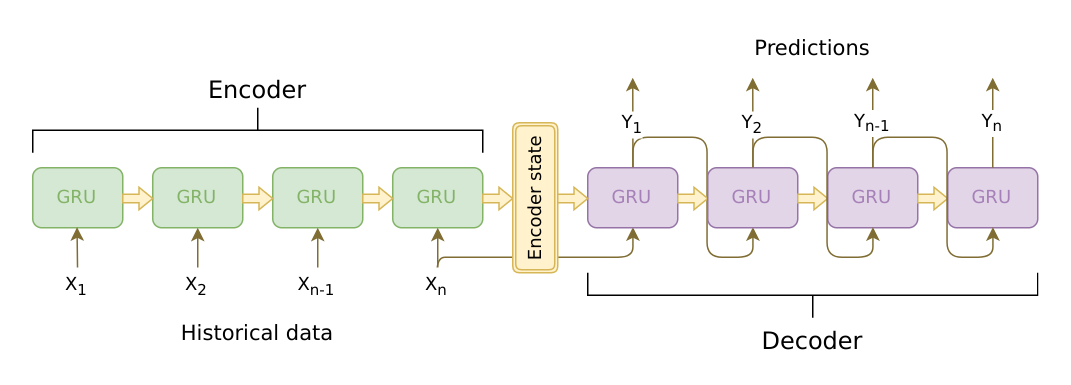
\includegraphics[width=\textwidth]{seq2seq}
	\caption*{Image source: \cite{seq2seq_eddy}}
\end{figure}
\end{itemize}

\section{Seq2seq with Attention}

\begin{itemize}
\item 
At each decoder step, it decides which source parts are more important

\item Concretely, at each $t,$:
	\begin{enumerate}[label=(\roman*)]
	\item
	Use previous token in RNN to update hidden state $h_t.$
	
	\item 
	Compute  $\score(h_t,s_k)$ between decoder hidden state $h_t$ and all encoder hidden states $s_1,\ldots,s_m;$
	
	\item 
	Compute attention weights: softmax attention scores;
	
	\item 
	Compute attention vector $a_t$: weighted sum of encoder states.
	
	\item 
	Use attention vector $a_t$ and hidden state $h_t$ in FNN to get output token.
	\end{enumerate}

\item Popular score functions:
	\begin{itemize}
	\item 
	Dot-product: $\score(h_t,s_k) = h_t^T s_k.$
	
	\item 
	Bilinear function: $\score(h_t,s_k) = h_t^T W s_k.$
	
	\item 
	Multi-layer perceptron: $\score(h_t,s_k) = v^T\tanh(W[h_t,s_k]).$
	\end{itemize}

\item Drawback: RNN is difficult to parallelize.

\begin{figure}[ht]
	\centering
	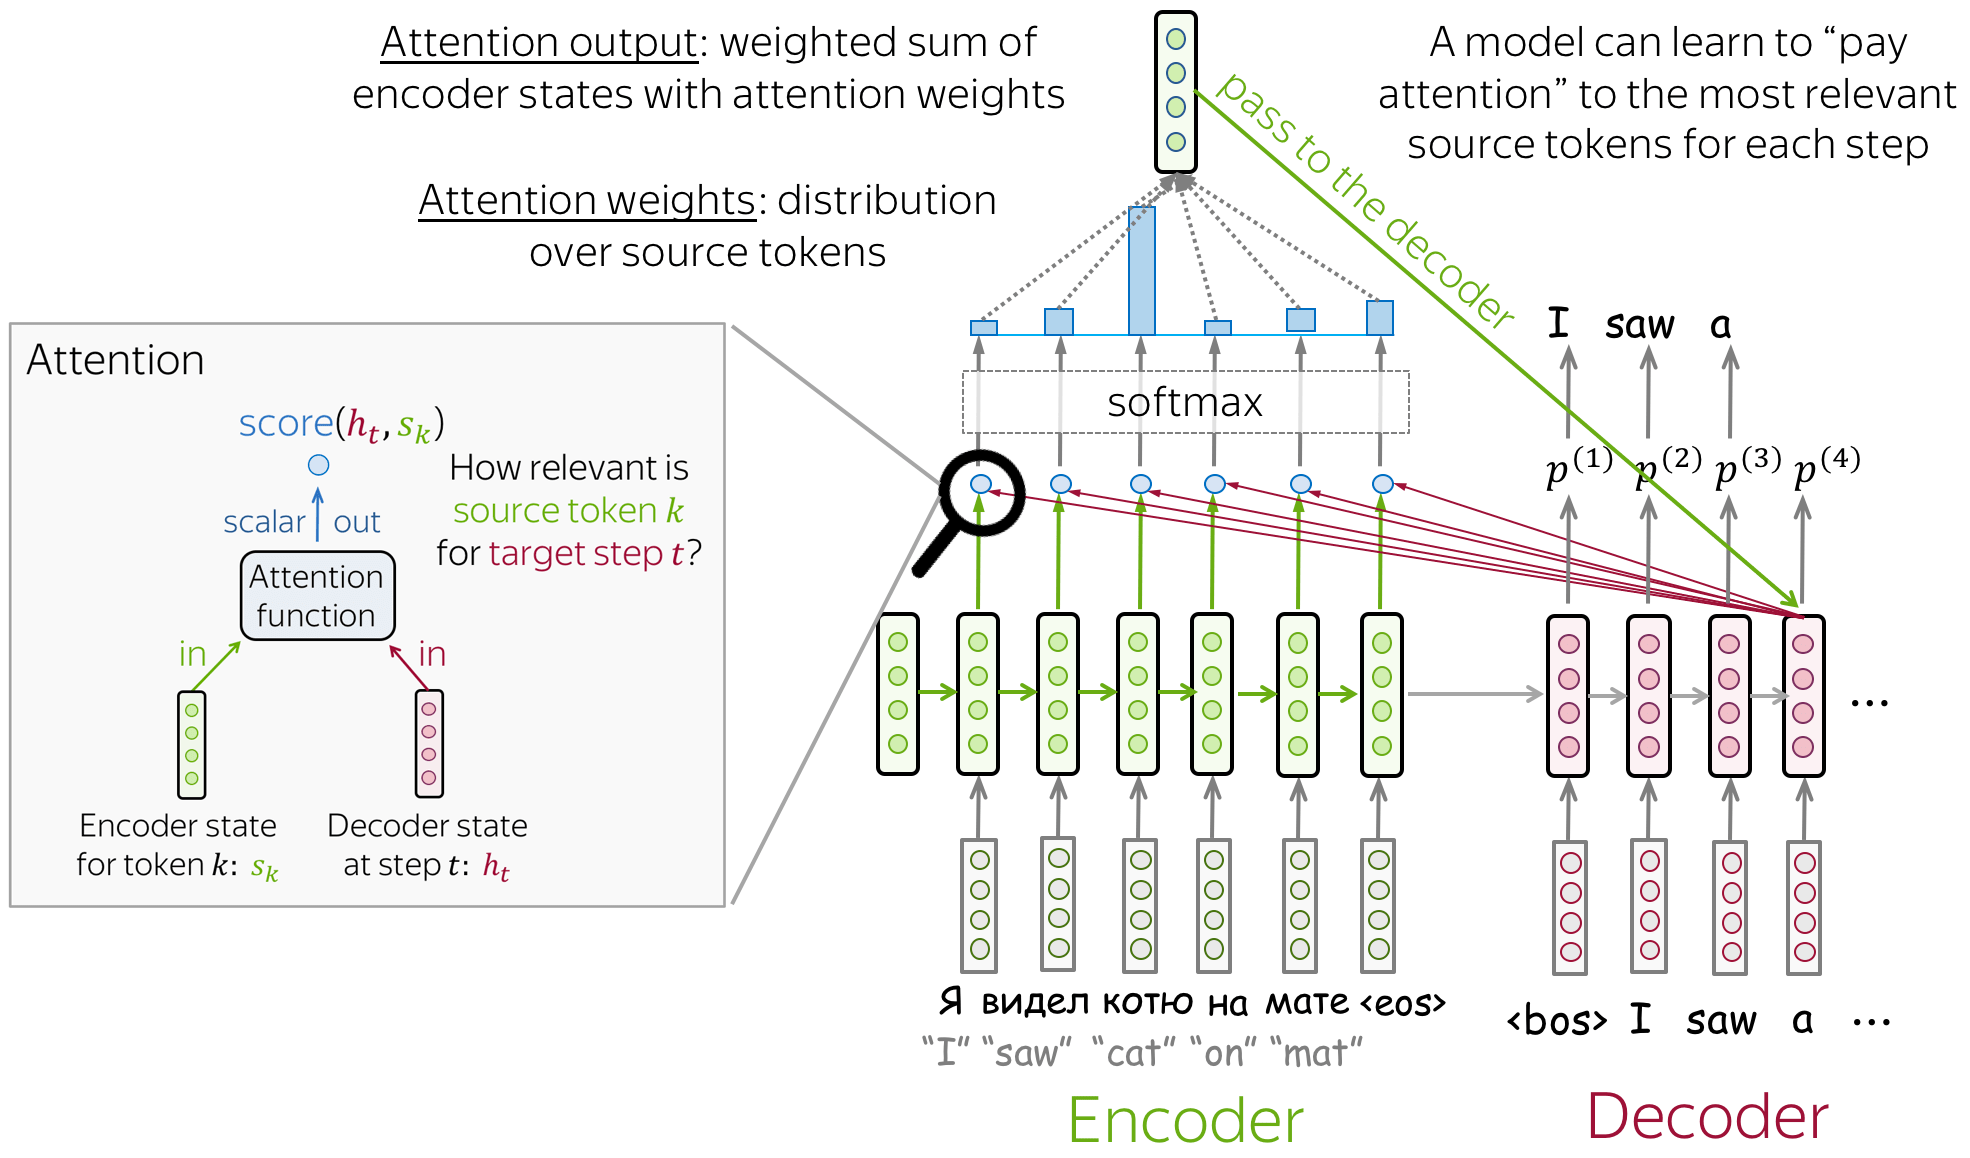
\includegraphics[width=\textwidth]{seq2seq_attention}
	\caption*{Image source: \cite{seq2seq_voita}}
\end{figure}
\end{itemize}
\chapter{Transformers}

\begin{itemize}
\item 
Encoding component is a stack (six in original paper) of encoders with same structure but different weights. Decoding component is a stack of decoders of the same number.

\item 
Encoders: Self-Attention \textrightarrow{} FNN
	\begin{itemize}
	\item 
	First encoder receives embedding of words.
	
	\item 
	Other encoders receive output of encoder directly below.
	\end{itemize}

\item 
Decoders: Self-Attention \textrightarrow{} Encoder-Decoder Attention \textrightarrow{} FNN
\end{itemize}

\section{Ingredients}
\subsection{Self-attention}
Process:
\begin{enumerate}
\item Create three vectors from each of the encoder’s input vectors: Query, Key, and Value vectors.

\item Note: in original paper, input vectors are in $\R^{512},$ and QKV vectors are in $\R^{64}.$

\item Self-attention score between $i$-th and $j$-th word is $q_i \cdot k_j$ for all $j.$

\item Divide scores by square root of dimension (8; this gives more stable gradients) and softmax.

\item Multiply each value vector $v_j$ by softmax scores.

\item Sum up the weighted value vectors. This is output of self-attention layer for $i$-th word.
\end{enumerate}
In matrix form, suppose our input is $X \in \R^{n \times d},$ where $n$ is the sequence length and $d$ is the embedding dimension. (So rows of $X$ are the inputs.) The QKV matrices are given by $W_Q, W_K, W_V \in \R^{d \times d_k}.$ Then the QKV vectors
\begin{align*}
    Q &= XW_Q \\
    K &= XW_K \\
    V &= XW_V
\end{align*}
are in $R^{n \times d_k}$
For each attention head, we have
\[ \att(Q,K,V) = \softmax\left(\frac{QK^T}{\sqrt{d_k}}\right) \times V \in \R^{n \times d_k}, \]
i.e., aggregate values weighted by attention.

\subsection{Multi-headed attention}
Do $h$ parallel attention heads, with different weight matrices for each head.
\[ \operatorname{MultiHead}(Q, K, V) = \operatorname{Concat}(\head_1, \ldots, \head_h) \times W_O, \]
where
\[ \head_i = \att(Q_i, K_i, V_i) \]
is output of each attention head and $W_O \in \R^{hd_k \times d}.$ Note that $\operatorname{MultiHead}(Q, K, V) \in \R^{n \times d}.$ 

\subsection{Positional encoding}
Transformers are permutation-invariant, so we add positional encoding to input embeddings.

\subsection{FNN}
Output of attention fed into FNN:
\[ \operatorname{FNN}(x) = \operatorname{ReLU}(xW_1 + b_1)W_2 + b_2. \]

\subsection{Residual connections \& layer normalization}
Each sub-layer (attention or feedforward) is followed by
\[ \layernorm(x + \operatorname{Sublayer}(x)). \]
Given $x \in \R^d,$ the layer norm is 
\[ \layernorm(x) = \frac{x - \mu}{\sqrt{\sigma^2 + \epsilon}} \cdot \gamma + \beta, \]
where
\begin{gather*}
    \mu = \frac{\sum x_i}{d} \text{ (mean over features)}\\
    \sigma^2 = \frac{\sum(x_i - \mu)^2}{d} \text{ (variance over features)}\\
    \gamma,\beta \text{: learned scaling and shifting parameters}\\
    \epsilon \text{: small constant to prevent division by zero}.
\end{gather*}

\section{Original Architecture}
Encoder Layer:
\begin{itemize}
    \item Input Embedding + Positional Encoding
    \item Multi-Head Self-Attention \textrightarrow{} Residual + Layer Norm
    \item Feed-Forward Network \textrightarrow{} Residual + Layer Norm
\end{itemize}
Decoder Layer:
\begin{itemize}
\item Masked Multi-Head Self-Attention (prevent peeking at future tokens)
\item Multi-Head Encoder-Decoder Attention \textrightarrow{} Residual + Layer Norm
\item Feed-Forward Network \textrightarrow{} Residual + Layer Norm
\end{itemize}

\section{Modern Architecture}
\begin{itemize}
    \item Input Embedding
    \item Layer Norm \textrightarrow{} Self-Attention \textrightarrow{} Residual
        \begin{itemize}
            \item Grouped-Query Attention
            \item Rotary Embeddings
        \end{itemize}
    \item Layer Norm \textrightarrow{} FNN \textrightarrow{} Residual
\end{itemize}

\subsection{Grouped-query attention}
\begin{itemize}
    \item Use same $W_K$ and $W_V$ across heads, and each head has its own $W_Q.$
    \item Better: divide heads into groups. Heads in the same group share $W_K$ and $W_V$
\end{itemize}

\subsection{Rotary positional embeddings (RoPE)}
\begin{itemize}
	\item Limitations of absolute positional embedding:
	\begin{itemize}
		\item Limited sequence length
		\item Independence of positional embedding, e.g./ difference between position 1 and 2 is the same as the difference between position 1 and 500
	\end{itemize}
    \item Alternative: \textit{relative positional embeddings} \cite{relposrep}
    \begin{itemize}
        \item Bias for positional offsets: use a bias to represent each possible positional offset
        \item Relative attention becomes:
        \begin{equation*}
            \att(Q,K,V)_i = \sum_{j=1}^{n}\softmax(e_{ij}) \times (x_jW_V + a_{ij}^V),
        \end{equation*}
        where
        \begin{equation*}
            e_{ij} = \frac{QK^T + x_iW_Q(a_{ij}^K)^T}{\sqrt{d_k}}.
        \end{equation*}
        \item Here, $a_{ij} \in \R^{1\times d_a}$ is a vector of relative positional weights, i.e.,
        \begin{gather*}
            a_{ij} = w_{\operatorname{clip}(j-i,k)}\\
            \operatorname{clip}(x,k) = \max(-k, \min(k,x)).
        \end{gather*}
        Calculate $w$ for both keys and values.
        \item Clipping allows scalability (i.e., arbitrarily long sequences)
        \item Limitations: slower; complicates key-value cache usage as each additional token changes the embedding for every other token.
    \end{itemize}
    \item For \textbf{RoPE} \cite{rotpos}, the intuition is to rotate each embedding by $m \theta,$ where $m$ is the position of the word in the sequence.
    \item Benefits:
        \begin{itemize}
            \item Scalability: adding new words does not change the embedding of previous words
            \item The dot product of the embeddings of two words does not depend on absolute position.
        \end{itemize}
    \item Mathematically, we first work in $\C^{d_k/2}.$ Let $M_j$ be the rotation matrix by $m \theta_j.$ Then the output of RoPE for the $m$-th word is just
    \begin{equation*}
        Q_m\Theta_m = Q_m \times
        \begin{pmatrix}
        M_1 & & & \\
        & M_2 & & \\
        & & \ddots & \\
        & & & M_{d_k/2}
        \end{pmatrix},
    \end{equation*}
    where $Q_m$ is the $m$-th row of $Q$ (i.e., query vector for $m$-th word).
    \item Do the same for key vector.
\end{itemize}

\section{Other Techniques}
\subsection{Sparse attention}
Instead of global autoregressive self-attention, use local autoregressive self-attention in some layers.

\subsection{Mixture of experts (MOE)}
\begin{itemize}
    \item Instead of a single monolithic feedforward layer in the transformer block, use a set of expert networks, and route the input to only a few of them.
    \item A router (a smaller FNN) calculates which experts to turn on.
    \item Could do model merging by doing a weighted average of experts using weights from the router.
\end{itemize}


\chapter{Fine-Tuning Techniques}

Full fine-tuning, of course, has the best performance but is computationally expensive. Need parameter-efficient fine-tuning (PEFT).

\begin{itemize}
    \item Adapter-based methods
    \begin{itemize}
        \item Adapters: small, trainable models inserted into pre-trained transformers.
        \item Freeze original model weights.
    \end{itemize}
    \item Instruction tuning
\end{itemize}

\section{Low-Rank Adaptation (LoRA)}
Introduced in \cite{lora}.
\begin{itemize}
    \item Intuition: only train low rank perturbations of the (selected) weight matrices.
    \item Let $W_0 \in \R^{d \times k}$ be a pre-trained weight matrix.
    \item Update: $W_0 + \Delta W = W_0 + BA,$ where $B \in \R^{d \times r}, A \in \R^{r \times d}, r \ll \min(d,k).$
    \item Advantages:
    \begin{itemize}
        \item Roughly converges to full fine-tuning as $r$ increases.
        \item No additional inference latency: when needing to switch to another downstream task, can recover $W_0$ by subtracting $BA,$ and then we can add a new $B'A'.$
    \end{itemize}
    \item Notes \cite{lora_notes}:
    \begin{itemize}
        \item Optimal placement highly dependent on the dataset and model architecture.
        \item For transformers, applying LoRA exclusively to attention layers provides the most stability and mitigates the risk of divergence.
        \item For MoE, applying LoRA to each expert individually boosts performance, but significantly increases memory usage. Applying to router gives limited success.
        \item Could optimize memory by using same $B$ across different $A.$
    \end{itemize}
\end{itemize}

\section{QLoRA}
Quantized LoRA, introduced in \cite{qlora}.

\subsection{4-bit NormalFloat Quantization}

\begin{itemize}
    \item Better quantization data type for normally distributed data.
    \item In general, for $k$-bit NormalFloat, equally divide the normal distribution into $2^k$ quantiles.
    \item Note: to ensure $0$ has an exact representation, actually divide the negative part into $2^{k-1}$ quantiles and the positive part into $2^{k-1} + 1$ quantiles, then remove one of the two overlapping zeros.
    \item Then
    \begin{equation*}
        X^{\nf 4} = \round\left(\frac{1}{\absmax(X^{\fp 32})} X^{\fp 32}\right) = \round(c^{\fp 32}X^{\fp 32}),
    \end{equation*}
    where $c^{\fp 32}$ is the \textit{quantization constant}.
\end{itemize}

\subsection{Block-wise Quantization}
\begin{itemize}
    \item One problem is quantization is that outliers severely impacts the scaling, and the full range of the lower precision data type may not be effectively used.
    \item Solution: Chunk the input tensor into blocks that are independently quantized, each with its own quantization constant.
\end{itemize}

\subsection{Double Quantization}
\begin{itemize}
    \item Helps reduce the memory footprint of quantization constants.
    \item Block-wise $k$-bit quantization for the quantization constants $c^{\fp 32}.$
    \item Gives $c^{\kbit}_2,$ with second level of quantization constants $c_1^{\fp 32}.$
\end{itemize}

\subsection{Implementation}
\begin{itemize}
    \item Recall: LoRA has
    \begin{equation*}
        Y = XW + XL_1L_2
    \end{equation*}
    for low rank matrices $L_i.$
    \item For QLoRA, do
    \begin{equation*}
        Y^{\bfl 16} = X^{\bfl 16}\doubleDequant(c_1^{\fp 32}, c_2^{\kbit}, W^{\nf 4}) + X^{\bfl 16}L_1^{\bfl 16}L_2^{\bfl 16},
    \end{equation*}
    where
    \begin{equation*}
        \doubleDequant(c_1^{\fp 32}, c_2^{\kbit}, W^{\nf 4}) = \dequant(\dequant(c_1^{\fp 32}, c_2^{\kbit}), W^{\nf 4}) = W^{\bfl 16}
    \end{equation*}
    \item Original paper \cite{qlora} uses $\fp 8$ for $c_2,$ block size of 64 for $W,$ and block size of 256 for $c_2.$
    \item Computations done in $\bfl 16$ and storage of $W$ in $\nf 4.$
\end{itemize}

\subsection{\texorpdfstring{\iat}{IA3}}
\begin{itemize}
    \item Introduced in \cite{ia3}, Infused Adapter by Inhibiting and Amplifying Inner Activations is intended to improve over LoRA.
    \item Notation: if $l \in \R^d$ and $A \in \R^{m \times d},$ then $(l \odot A)_{ij} = l_jA_{ij},$ i.e., element-wise multiplication of $l$ and rows of $A.$
    \item Learned vectors $l_v,l_k,l_f.$
    \item Attention layer:
    \begin{equation*}
        \softmax\left(\frac{Q(l_k \odot K^T)}{\sqrt{d_k}}\right) \times (l_v \odot V)
    \end{equation*}
    \item Feedforward layer:
    \begin{equation*}
        (l_f \odot \gamma(W_1x))W_2,
    \end{equation*}
    where $\gamma$ is the FFN nonlinearity.
\end{itemize}
\chapter{Fourier Transform}
\begin{itemize}
\item 
Let $x(t)$ be a complex-valued function. Then its Fourier transform is 
\[ X(\omega) = \int_{-\infty}^\infty x(t)e^{-i\omega t}\,dt. \]
The inverse Fourier transform is
\[ x(t) = \frac{1}{2\pi} \int_{-\infty}^\infty X(\omega)e^{i\omega t}\,d\omega. \]

\item 
For a sequence of discrete time signals, use discrete-time Fourier transform:
\[ X(\omega) = \sum_{-\infty}^\infty x[n]e^{-i\omega n}. \]
The output is continuous in $\omega$ and periodic. The inverse DTFT is:
\[ x[n] = \frac{1}{2\pi} \int_{2\pi} X(\omega)e^{i\omega n}\,d\omega. \]

\item
Discrete Fourier transform converts a finite sequence of equally-spaced samples of a function into a same-length sequence of equally-spaced samples of the DTFT. It is given by
\begin{align*} X[k] &= \sum_{n=0}^{N-1} x[n]e^{-2\pi i kn/N} \\&= \sum_{n=0}^{N-1} x[n]W_N^{kn},
\end{align*}
where $W_N = e^{-2\pi i/N}.$
The inverse transform is given by 
\[ \frac{1}{N} \sum_{k=0}^{N-1} X[k]W^{-kn}_N.\]

\item 
The fast Fourier transform is based on the idea that the $N$-th roots of unity $W_N^k$ have nice properties when $N$ is a power of $2.$ In vector form,
\[ \mathbf{X}[k] = \mathbf{W_N}\mathbf{x}[n], \]
where $W_N = V(W_N^0,\ldots,W_N^{N-1})$ is a Vandermonde matrix. The computational complexity is $O(N\log{N})$ vs.\ $O(N^2)$ of definition of DFT.

\item 
Limitation of Fourier transform is that it lacks temporal resolution. A way to overcome this is the short-time Fourier transform.
	\begin{itemize}
	\item 
	Continuous case:
	\[ \STFT\{x(t)\}(\tau, \omega) = \int_{-\infty}^{\infty} x(t)w(t - \tau)e^{-i\omega t}\,dt, \] where $w$ is the window function, usually Hann or Gaussian window.
	
	\item 
	Discrete case:
	\[ \STFT\{x[n]\}(k, \omega) = \sum_{n=-\infty}^{\infty} x[n]w[n-k]e^{-i\omega n}. \]
	\end{itemize}
Uncertainty principle: there is a trade-off between temporal and frequency resolution.

\begin{figure}[ht]
	\centering
	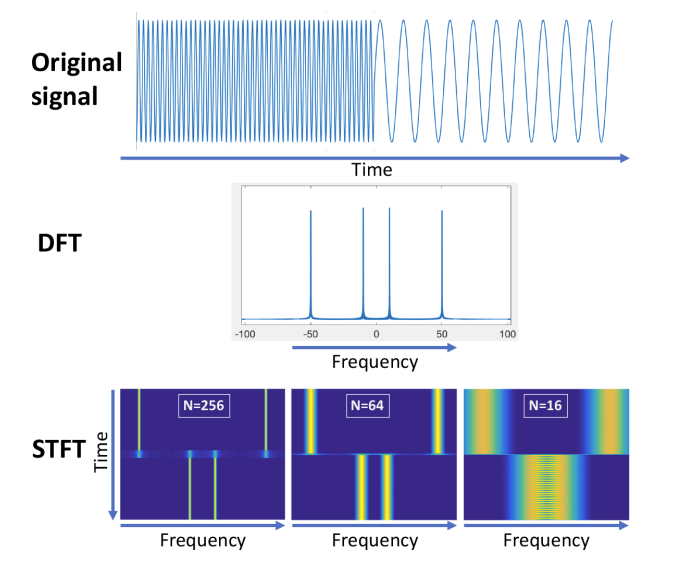
\includegraphics[width=10cm]{fourier_uncertainty}
	\caption*{Image source: \cite{fourier_qiml}}
\end{figure}

\item 
Spectrograms:
	\begin{itemize}
	\item 
	Divide a time-domain signal into segments of equal length.
	
	\item 
	Apply FFT to each segment, transforming the data from the time domain to the frequency domain.
	
	\item 
	Each segment corresponds to vertical line in spectogram.
	
	\item 
	For window width $w,$ $\text{spectogram}(t) = |\STFT(t)|^2.$
	\end{itemize}

\item 
Nyquist–Shannon sampling theorem
	\begin{itemize}
	\item 
	Sampling rate must be at least twice the bandwidth of the signal to avoid aliasing.
	
	\item 
	Let $x(t)$ have Fourier transform $X(f).$ Suppose $X_{1/T}(f)$ is the DTFT of sample sequence $x[n].$ 
	
	\item 
	For DTFT, copies of $X_f$ are shifted by multiples of the sampling rate $f_s$ and added.
	
	\item
	If Nyquist–Shannon is not satisfied, copies will overlap.
	
	\item 
	Any frequency component above $f_s/2$ is indistinguishable from a lower-frequency component (i.e., alias).
	\end{itemize}
\end{itemize}

\nocite{*}
\bibliographystyle{plain}
\bibliography{bib/bibliography.bib}

\end{document}